%!TEX program = xelatex
\documentclass[10pt, compress]{beamer}
\usetheme[titleprogressbar]{m}

\usepackage{booktabs}
\usepackage[scale=2]{ccicons}
\usepackage{minted}

\usepgfplotslibrary{dateplot}

\usemintedstyle{trac}

\setbeamertemplate{caption}[numbered]
\setbeamertemplate{theorems}[numbered]
\newtheorem{crl}{Corollary}[theorem]
\newtheorem*{solution*}{Solution}

\usepackage{algorithm}
\usepackage[noend]{algpseudocode}

\usepackage{version}
%\excludeversion{proof}
%\excludeversion{solution*}

\usepackage{mathtools}
\usepackage{multicol}
\usepackage{qtree}

\usepackage{tikz}

\makeatletter
\def\old@comma{,}
\catcode`\,=13
\def,{%
	\ifmmode%
	\old@comma\discretionary{}{}{}%
	\else%
	\old@comma%
	\fi%
}
\makeatother

\title{CSCI 3190 Tutorial of Week 03}
\subtitle{Relations}
\author{LI Haocheng}
\institute{Department of Computer Science and Engineering}

\begin{document}

\maketitle

\begin{frame}[fragile]
	\frametitle{Inverse Relation}
	\begin{columns}
		\begin{column}{.6\linewidth}
			Let $R$ be a relation from a set $A$ to a set $B$.
			\begin{definition}
				The \textbf{inverse relation} from $B$ to $A$, denoted by $R^{-1}$, is the set of ordered pairs $\{(b, a) \mid (a, b) \in R \}$.
			\end{definition}
			\begin{definition}
				The \textbf{complementary relation} $\bar{R}$ is the set of ordered pairs $\{(a, b) \mid (a, b) \notin R \}$.
			\end{definition}
		\end{column}
		\begin{column}{.4\linewidth}
			\begin{example}
				Let $R$ be the relation $R = \{(a, b) \mid a < b\}$ on the set of integers. Find \begin{enumerate}
					\onslide<1->\item $R^{-1}$ \onslide<2>$= \{(a, b) \mid a > b\}$
					\onslide<1->\item $\bar{R}$ \onslide<2>$= \{(a, b) \mid a \ge b\}$
				\end{enumerate}
			\end{example}
		\end{column}
	\end{columns}
	
\end{frame}

\begin{frame}[allowframebreaks]
	\frametitle{Tree}
	\begin{example}
		\begin{enumerate}[(a)]
			\item Show that the sum of the degrees of the vertices of a tree with $n$ vertices is $2n-2$.
			\item For $n \ge 2$, let $d_1, d_2, \cdots , d_n$ be $n$ positive integers such that $d_1 + d_2 + \cdots + d_n = 2n -2$. Show that there
			exists a tree whose vertices have degrees $d_1, d_2, \cdots, d_n$. 
		\end{enumerate}
	\end{example}
	\newpage
	\begin{proof}
		\begin{enumerate}[(a)]
			\item A $n$-vertex tree has $n-1$ edges so that the total degree is $2n - 2$.
			\item For $n = 2$, this is trivial. Suppose $\forall$ positive $d_i$ such that $\Sigma_{i = 1}^{n - 1} d_i = 2n - 4$, $\exists$ a tree $T^\prime$ whose vertices have degrees $d_1, d_2, \cdots, d_{n - 1}$. Then $\forall$ positive $d_i$ such that $\Sigma_{i = 1}^{n} d_i = 2n - 2$, since $d_i$ cannot be all greater than 1 or less than 2, without loss of generality, let $d_{n - 1} > 1, d_n = 1$. Hence we can remove $d_n$ and subtract $d_{n - 1}$ by 1 so that $\Sigma_{i = 1}^{n - 1} d_i = 2n - 4$ and we can find a tree $T^\prime$. After that we can add vertex $d_n$ as a leaf of $d_{n - 1}$ to build the final tree $T$.
		\end{enumerate}
	\end{proof}
\end{frame}

\begin{frame}[fragile]
	\frametitle{Traversal}
	\begin{columns}
		\begin{column}{.5\linewidth}
			\onslide<1->\begin{example}
				Construct a DFS and a BFS traversal for the graphs in Figure starting with node B as the root.
			\end{example}
			\onslide<2>\begin{solution*}
				\begin{enumerate}[(a)]
					\item \begin{description}
						\item[DFS] B, A, C, F, D, E
						\item[BFS] B, A, C, D, E, F
					\end{description}
					\item \begin{description}
						\item[DFS] B, A, D, E, C
						\item[BFS] B, A, C, D, E
					\end{description}
				\end{enumerate}
			\end{solution*}
		\end{column}
		\onslide<1->\begin{column}{.5\linewidth}

		\end{column}
	\end{columns}
\end{frame}

\begin{frame}[allowframebreaks]
	\frametitle{Traversal}
	\begin{example}
		\begin{enumerate}[(a)]
			\item Construct a binary tree with 7 vertices of which the preorder traversal is the same as its inorder traversal. Give its postprder traversal and preorder traversal.
			\item Construct a binary tree with 8 vertices of which the postorder traversal is the same as its inorder traversal. Give its postprder traversal and preorder traversal.
			\item Construct a binary tree of which th preorder travelsal is the same as its postorder travelsal.
		\end{enumerate}
	\end{example}
	\begin{solution*}
		\begin{columns}
			\begin{column}{.4\linewidth}
				\begin{enumerate}
					\item See Figure \ref{f-4-1}.
					\begin{description}
						\item[Postorder] 7654321
						\item[Preorder] 1234567
					\end{description}
					\item See Figure \ref{f-4-2}.
					\begin{description}
						\item[Postorder] 87654321
						\item[Preorder] 12345678
					\end{description}
					\item See Figure \ref{f-4-3}.
					\begin{figure}
						\centering
						\begin{tikzpicture}
						\node[draw](z){1};
						\end{tikzpicture}
						\caption{A Tree $T$}
						\label{f-4-3}
					\end{figure}
				\end{enumerate}
			\end{column}
			\begin{column}{.3\linewidth}
				\begin{figure}
					\centering
					\begin{tikzpicture}
					\node[draw](z){1}
					[sibling distance=7mm] 
					[level distance=7mm]
					child[missing]
					child{
						node[draw]{2} 
						child[missing] 
						child{
							node[draw]{3} 
							child[missing] 
							child{
								node[draw]{4} 
								child[missing] 
								child{
									node[draw]{5} 
									child[missing] 
									child{
										node[draw]{6} 
										child[missing] 
										child{
											node[draw]{7}}}}}}};
					\end{tikzpicture}
					\caption{A Tree $T$}
					\label{f-4-1}
				\end{figure}
			\end{column}
			\begin{column}{.3\linewidth}
				\begin{figure}
					\centering
					\begin{tikzpicture}
					\node[draw](z){1}
					[sibling distance=7mm] 
					[level distance=7mm]
					child{
						node[draw]{2} 
						child{
							node[draw]{3} 
							child{
								node[draw]{4} 
								child{
									node[draw]{5} 
									child{
										node[draw]{6} 
										child{
											node[draw]{7}
											child{
												node[draw]{8}
												child[missing] 
											}
											child[missing] 
										}
										child[missing] 
									}
									child[missing] 
								}
								child[missing] 
							}
							child[missing] 
						}
						child[missing] 
					}
					child[missing];
					\end{tikzpicture}
					\caption{A Tree $T$}
					\label{f-4-2}
				\end{figure}
			\end{column}
		\end{columns}
	\end{solution*}
\end{frame}

\begin{frame}[fragile]
	\frametitle{Complexity}
	\onslide<1->\begin{example}
		\begin{enumerate}
			\item Show that $f(n) = 3^n = O(n!)$.
			\item Show that $f(n) = 4^n = O(n!)$.
		\end{enumerate}
	\end{example}
	\onslide<2>\begin{solution*}
		\begin{enumerate}
			\item $\exists N = 0, \exists C = 5, \forall n \ge N, 3^n < C(n!)$.
			\item $\exists N = 0, \exists C = 11, \forall n \ge N, 4^n < C(n!)$.
		\end{enumerate}
	\end{solution*}
\end{frame}

\begin{frame}[allowframebreaks]
	\frametitle{Longest Common Subsequence}
	\begin{example}
		\begin{enumerate}[(a)]
			\item Find the longest common subsequence between $\alpha = \mathtt{abcbdaccdb}$ and $\beta = \mathtt{bbcad}$ by constructing a table $len$ where $len[i, j]$ is the length of the longest common subsequence between $\alpha[1]\alpha[2]\cdots\alpha[i]$ and $\beta[1]\beta[2]\cdots\beta[j]$ where $i = 1\cdots 10$ and $j = 1\cdots 5$.
			\item From the table $len$, find all the longest common subsequences between $\alpha$ and $\beta$. For each of the longest common subsequences, show how it can be found from the table.
		\end{enumerate}
	\end{example}
	\newpage
	\begin{solution*}
		\begin{table}
			\centering
			\caption{The Table $len$}
			\label{t-6}
			\begin{tabular}{c|ccccccccccc}
				\toprule 
				& 0 & a & b & c & b & d & a & c & c & d & b \\ 
				\midrule 
				0 & 0 & 0 & 0 & 0 & 0 & 0 & 0 & 0 & 0 & 0 & 0 \\ 
				b & 0 & 0 & \alert{1} & 1 & 1 & 1 & 1 & 1 & 1 & 1 & 1 \\ 
				b & 0 & 0 & 1 & 1 & \alert{2} & 2 & 2 & 2 & 2 & 2 & 2 \\ 
				c & 0 & 0 & 1 & \alert{2} & 2 & 2 & 2 & \alert{3} & 3 & 3 & 3 \\ 
				a & 0 & 1 & 1 & 2 & 2 & 2 & \alert{3} & 3 & 3 & 3 & 3 \\ 
				d & 0 & 1 & 1 & 2 & 2 & 3 & 3 & 3 & 3 & \alert{4} & 4 \\ 
				\bottomrule 
			\end{tabular}
		\end{table}
	\end{solution*}
\end{frame}

\begin{frame}[fragile]
	\frametitle{Euler Path}
	\onslide<1->\begin{columns}
		\begin{column}{.5\linewidth}
			\begin{example}
				Determine whether the given graph has an
				Euler circuit. Construct such a circuit when one exists. If
				no Euler circuit exists, determine whether the graph has an
				Euler path and construct such a path if one exists.
			\end{example}
		\end{column}
		\begin{column}{.5\linewidth}
			\begin{figure}
				\centering
				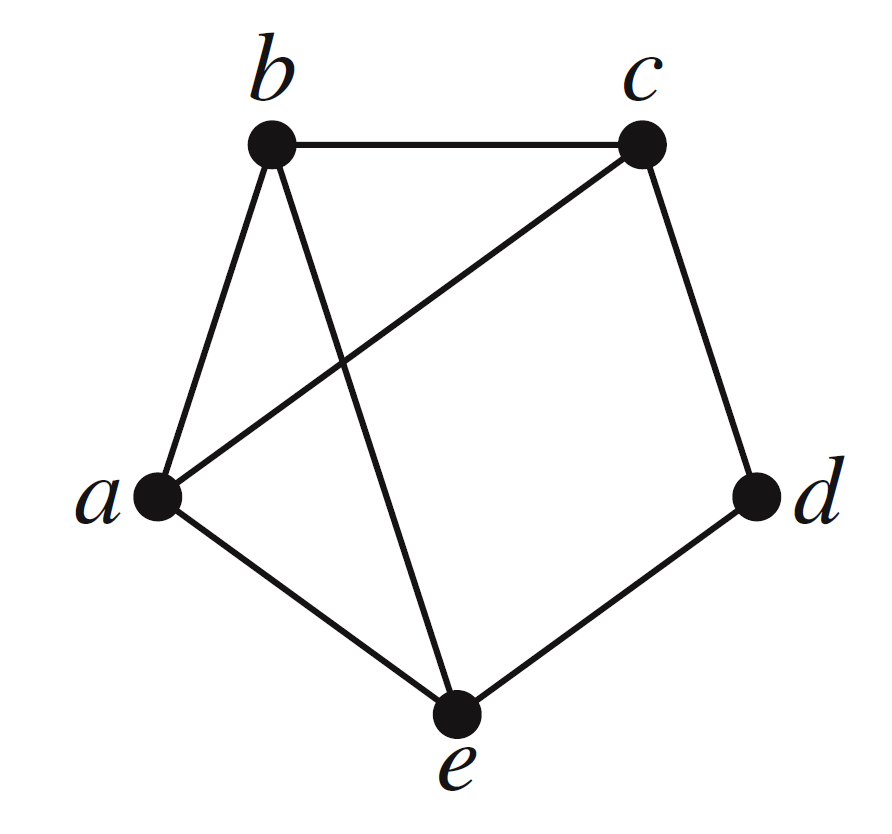
\includegraphics[width=.6\linewidth]{f-10-5-e-1}
			\end{figure}
		\end{column}
	\end{columns}
	\onslide<2>\begin{solution*}
		Neither.
	\end{solution*}
\end{frame}

\begin{frame}[fragile]
	\frametitle{Euler Circuit}
	\onslide<1->\begin{columns}
		\begin{column}{.5\linewidth}
			\begin{example}
				Determine whether the given graph has an
				Euler circuit. Construct such a circuit when one exists. If
				no Euler circuit exists, determine whether the graph has an
				Euler path and construct such a path if one exists.
			\end{example}
		\end{column}
		\begin{column}{.5\linewidth}
			\begin{figure}
				\centering
				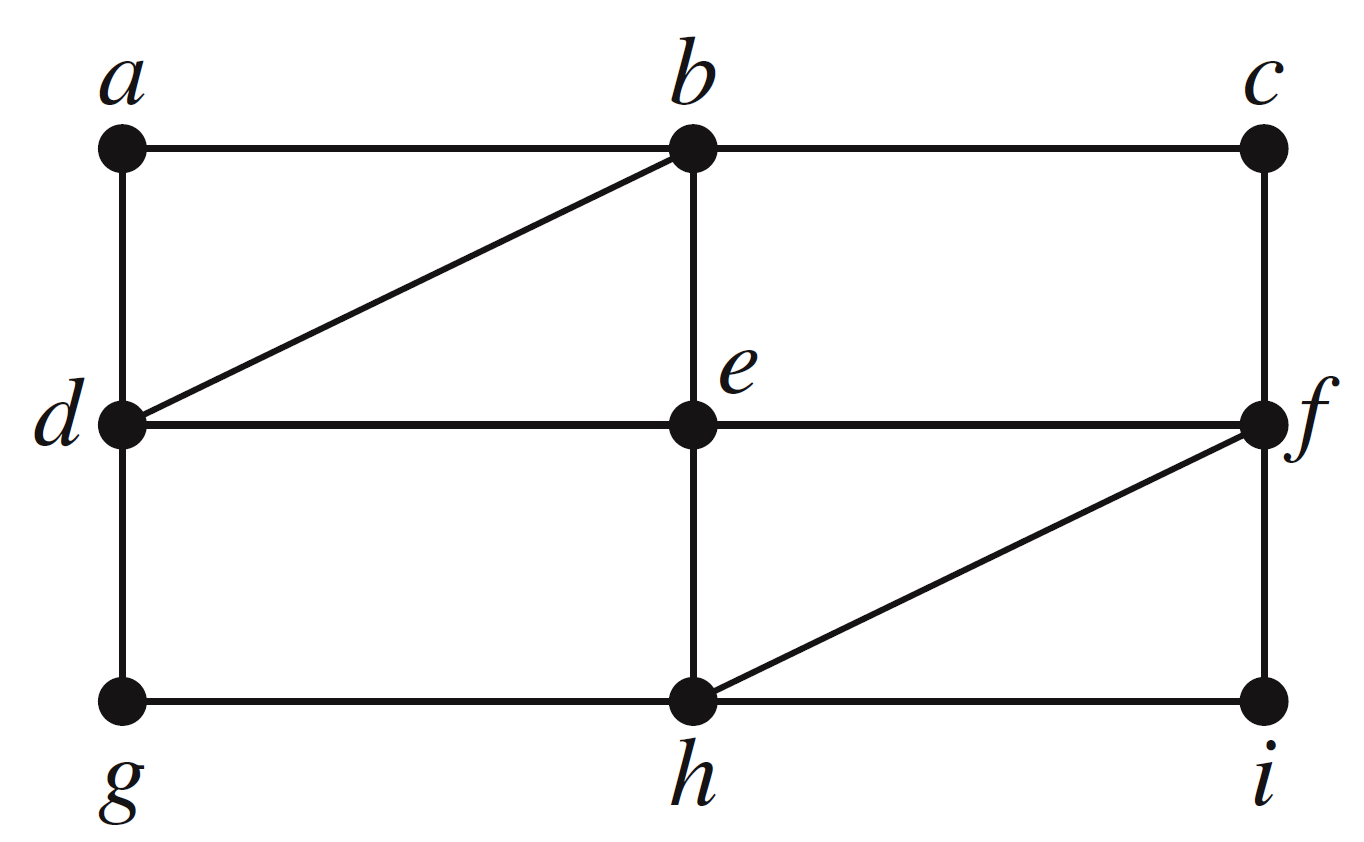
\includegraphics[width=.8\linewidth]{f-10-5-e-2}
			\end{figure}
		\end{column}
	\end{columns}
	\onslide<2>\begin{solution*}
		$a, b, c, f, e, b, d, e, h, f, i, h, g, d, a.$
	\end{solution*}
\end{frame}

\begin{frame}[fragile]
	\frametitle{Hamilton Path}
	\onslide<1->\begin{columns}
		\begin{column}{.5\linewidth}
			\begin{example}
				Which of the simple graphs in Figure have a Hamilton circuit or, if not, a Hamilton path?
			\end{example}
		\end{column}
		\begin{column}{.5\linewidth}
			\begin{figure}
				\centering
				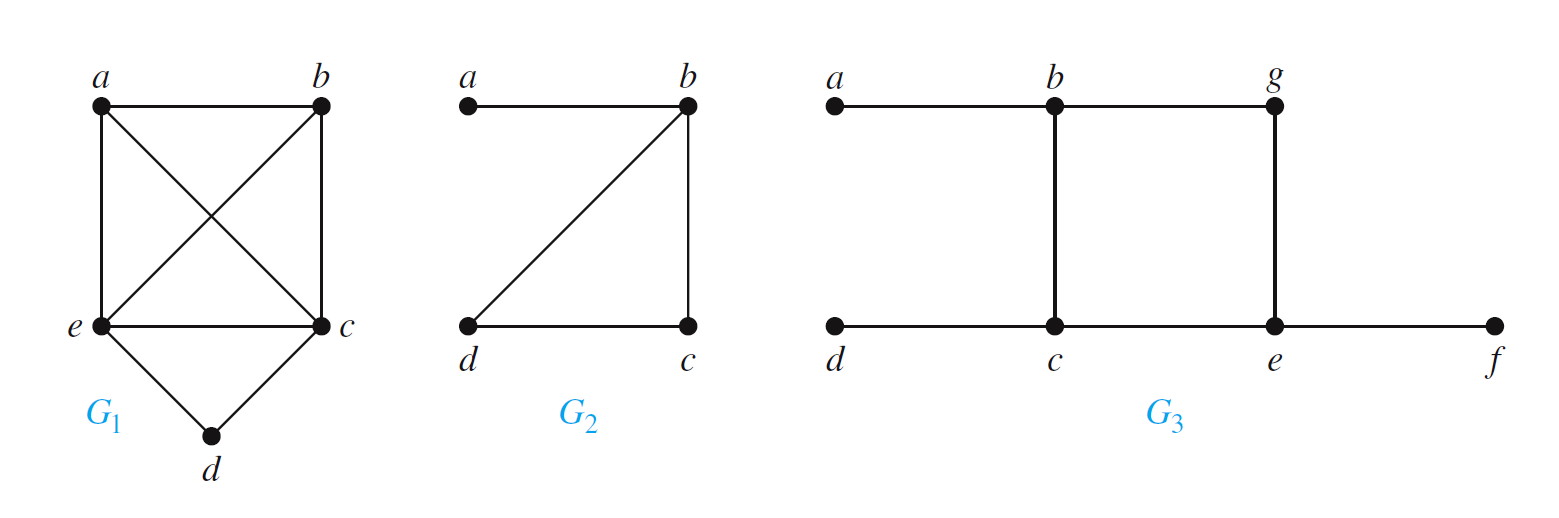
\includegraphics[width=\linewidth]{f-10-5-10}
			\end{figure}
		\end{column}
	\end{columns}
	\onslide<2>\begin{solution*}
		$G_1$ has a Hamilton circuit: $a, b, c, d, e, a$. There is no Hamilton circuit in $G_2$ (this can
		be seen by noting that any circuit containing every vertex must contain the edge $\{a, b\}$ twice),
		but $G_2$ does have a Hamilton path, namely, $a, b, c, d$. $G_3$ has neither a Hamilton circuit nor a
		Hamilton path, because any path containing all vertices must contain one of the edges $\{a, b\}, \{e, f\}$, and $\{c, d\}$ more than once.
	\end{solution*}
\end{frame}

\begin{frame}[fragile]
	\frametitle{Hamilton Circuit}
	\onslide<1->\begin{columns}
		\begin{column}{.5\linewidth}
			\begin{example}
				Show that neither graph displayed in Figure has a Hamilton circuit.
			\end{example}
		\end{column}
		\begin{column}{.5\linewidth}
			\begin{figure}
				\centering
				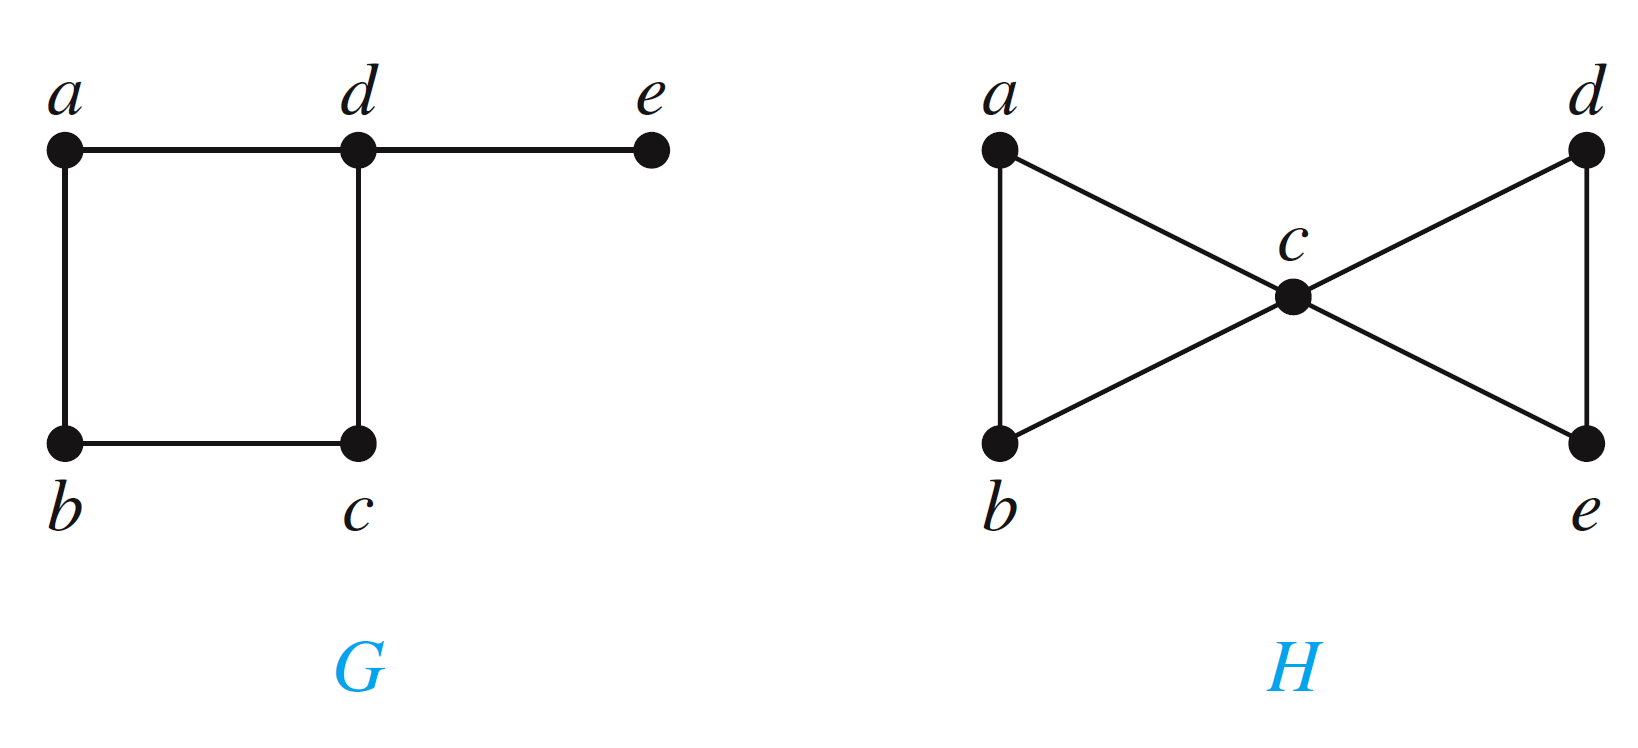
\includegraphics[width=\linewidth]{f-10-5-11}
			\end{figure}
		\end{column}
	\end{columns}
	\onslide<2>\begin{solution*}
		There is no Hamilton circuit in $G$ because $G$ has a vertex of degree one, namely, $e$. Now consider $H$. Because the degrees of the vertices $a, b, d$, and $e$ are all two, every edge incident with these vertices must be part of any Hamilton circuit. It is now easy to see that no Hamilton circuit can exist in $H$, for any Hamilton circuit would have to contain four edges incident with c, which is impossible.
	\end{solution*}
\end{frame}

\begin{frame}[fragile]
	\frametitle{Shortest Path}
	\onslide<1->\begin{columns}
		\begin{column}{.5\linewidth}
			\begin{example}
				Find the length of a shortest path between $a$
				and $z$ in the given weighted graph.
			\end{example}
		\end{column}
		\begin{column}{.5\linewidth}
			\begin{figure}
				\centering
				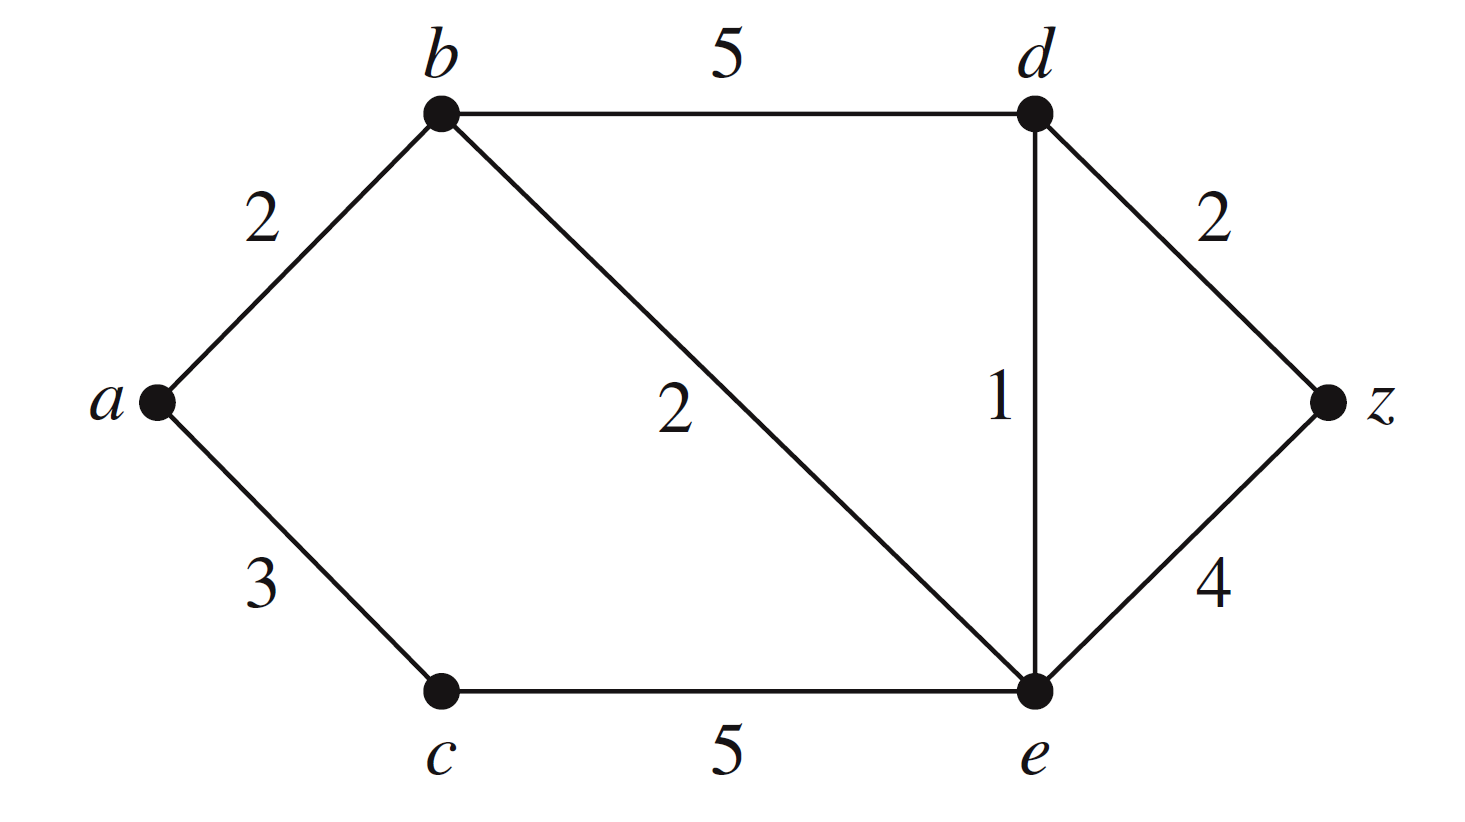
\includegraphics[width=\linewidth]{f-10-6-e-2}
			\end{figure}
		\end{column}
	\end{columns}
	\onslide<2>\begin{solution*}
		\begin{equation}
			2 + 2 + 1 + 2 = 7.
		\end{equation}
	\end{solution*}
\end{frame}

\begin{frame}[fragile]
	\frametitle{Newark}
	\onslide<1->\begin{columns}
		\begin{column}{.5\linewidth}
			\begin{example}
				Find a shortest route in distance between Newark and
				Camden, and between Newark and Cape May, using
				these roads.
			\end{example}
		\end{column}
		\begin{column}{.5\linewidth}
			\begin{figure}
				\centering
				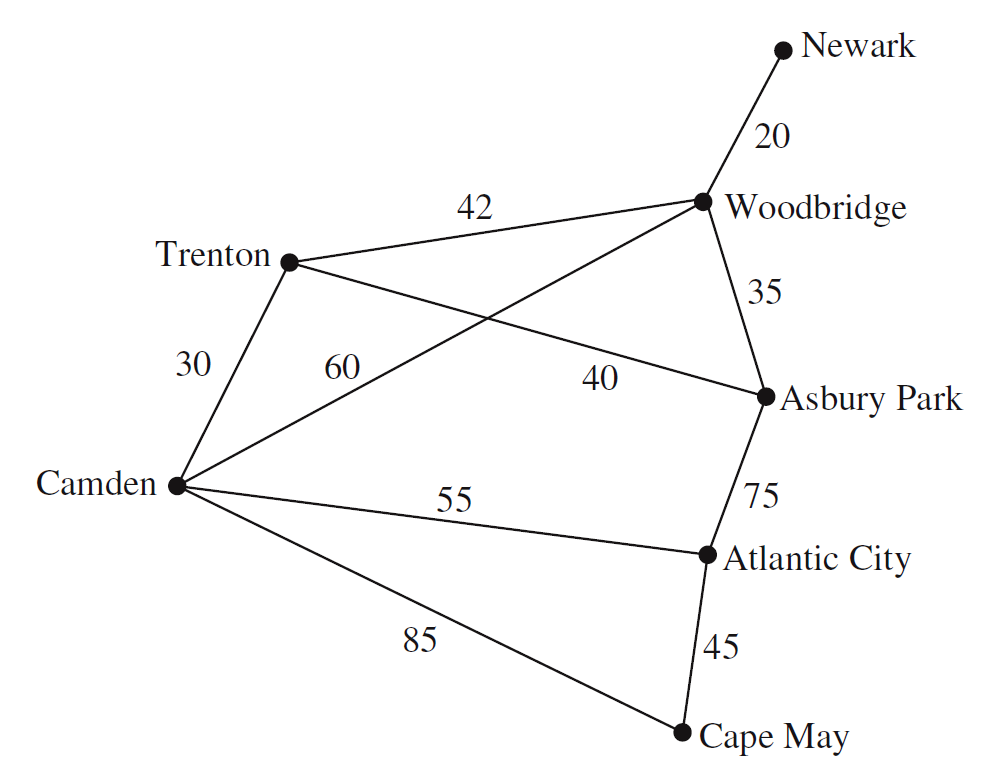
\includegraphics[width=\linewidth]{f-10-6-e-17-a}
			\end{figure}
		\end{column}
	\end{columns}
	\onslide<2>\begin{solution*}
		\begin{description}
			\item[Camden] 80
			\item[Cape May] 165
		\end{description}
	\end{solution*}
\end{frame}

\plain{Questions?}

\end{document}
